\documentclass[10pt]{beamer}
\usepackage[italian]{babel}
%\usepackage[utf8]{inputenc}

\usetheme{metropolis}
\usepackage{appendixnumberbeamer}

\usepackage{booktabs}
\usepackage[scale=2]{ccicons}

\usepackage{pgfplots}
\usepgfplotslibrary{dateplot}

\usepackage{listings}
\lstset{breaklines=true}

\usepackage[outputdir=out]{minted}

\usepackage{xspace}
\newcommand{\themename}{\textbf{\textsc{metropolis}}\xspace}
\newcommand{\circa}{$\sim$ }

\title{Moving to the Cloud}
\subtitle{The SeismoCloud case}
\date{}
\author{Enrico Bassetti}
\institute{Cloud Computing course \\ Sapienza, University of Rome}
%\titlegraphic{\hfill\includegraphics[height=1.5cm]{.png}}

\begin{document}

\setbeamertemplate{frame footer}{Moving to the Cloud: the SeismoCloud case - Cloud Computing @ Sapienza, University of Rome}

\maketitle

\begin{frame}{Roadmap}
  \setbeamertemplate{section in toc}[sections numbered]
  \tableofcontents[hideallsubsections]
\end{frame}


\section{Introduction to SeismoCloud}

\begin{frame}{Introduction to SeismoCloud}
SeismoCloud is an \textit{early warning system} for earthquakes based on a low
cost sismometers' network.

The goal is to warn residents about an incoming earthquake \textbf{once it
emerged on the epicenter}, within a margin of 5 \circa 20 seconds.

\vspace{1em}
\centering

\includegraphics[keepaspectratio=true,height=40pt]{dipartimentologo}

\includegraphics[keepaspectratio=true,height=40pt]{dipartimento}
\hspace{1em}

\includegraphics[keepaspectratio=true,height=40pt]{ingv}

\end{frame}


\begin{frame}{Introduction to SeismoCloud: map}
\centering
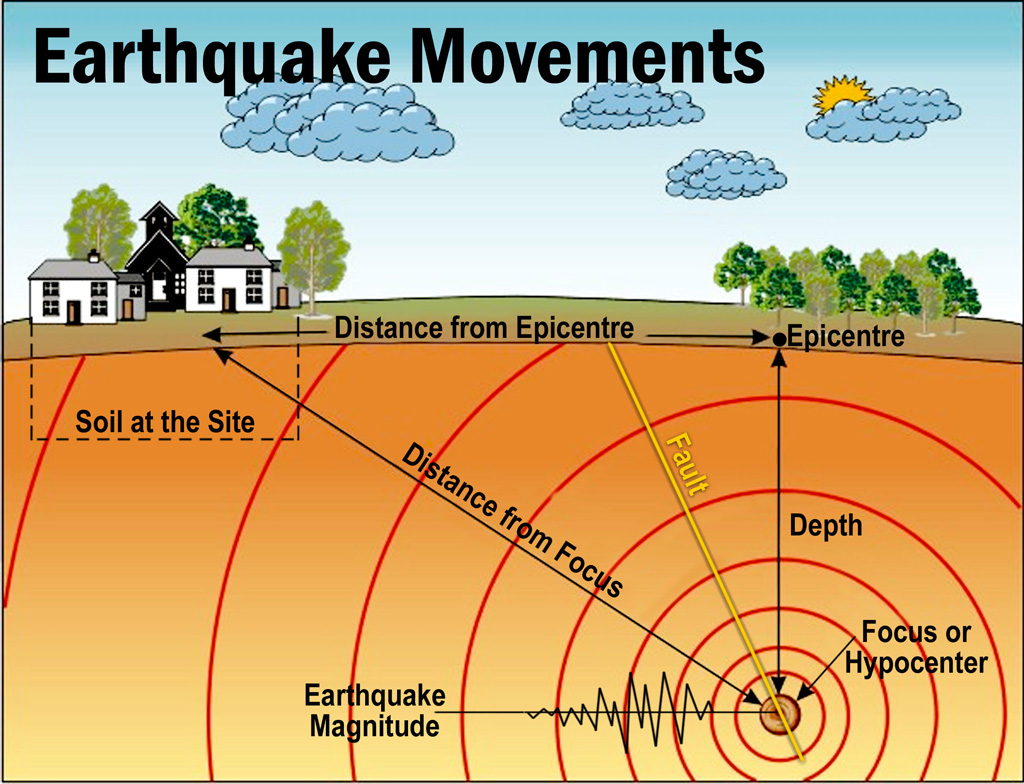
\includegraphics[keepaspectratio=true,width=0.85\textwidth]{earthquake-points}
\end{frame}



\section{Current architecture}

\begin{frame}{Current SeismoCloud architecture}
\centering
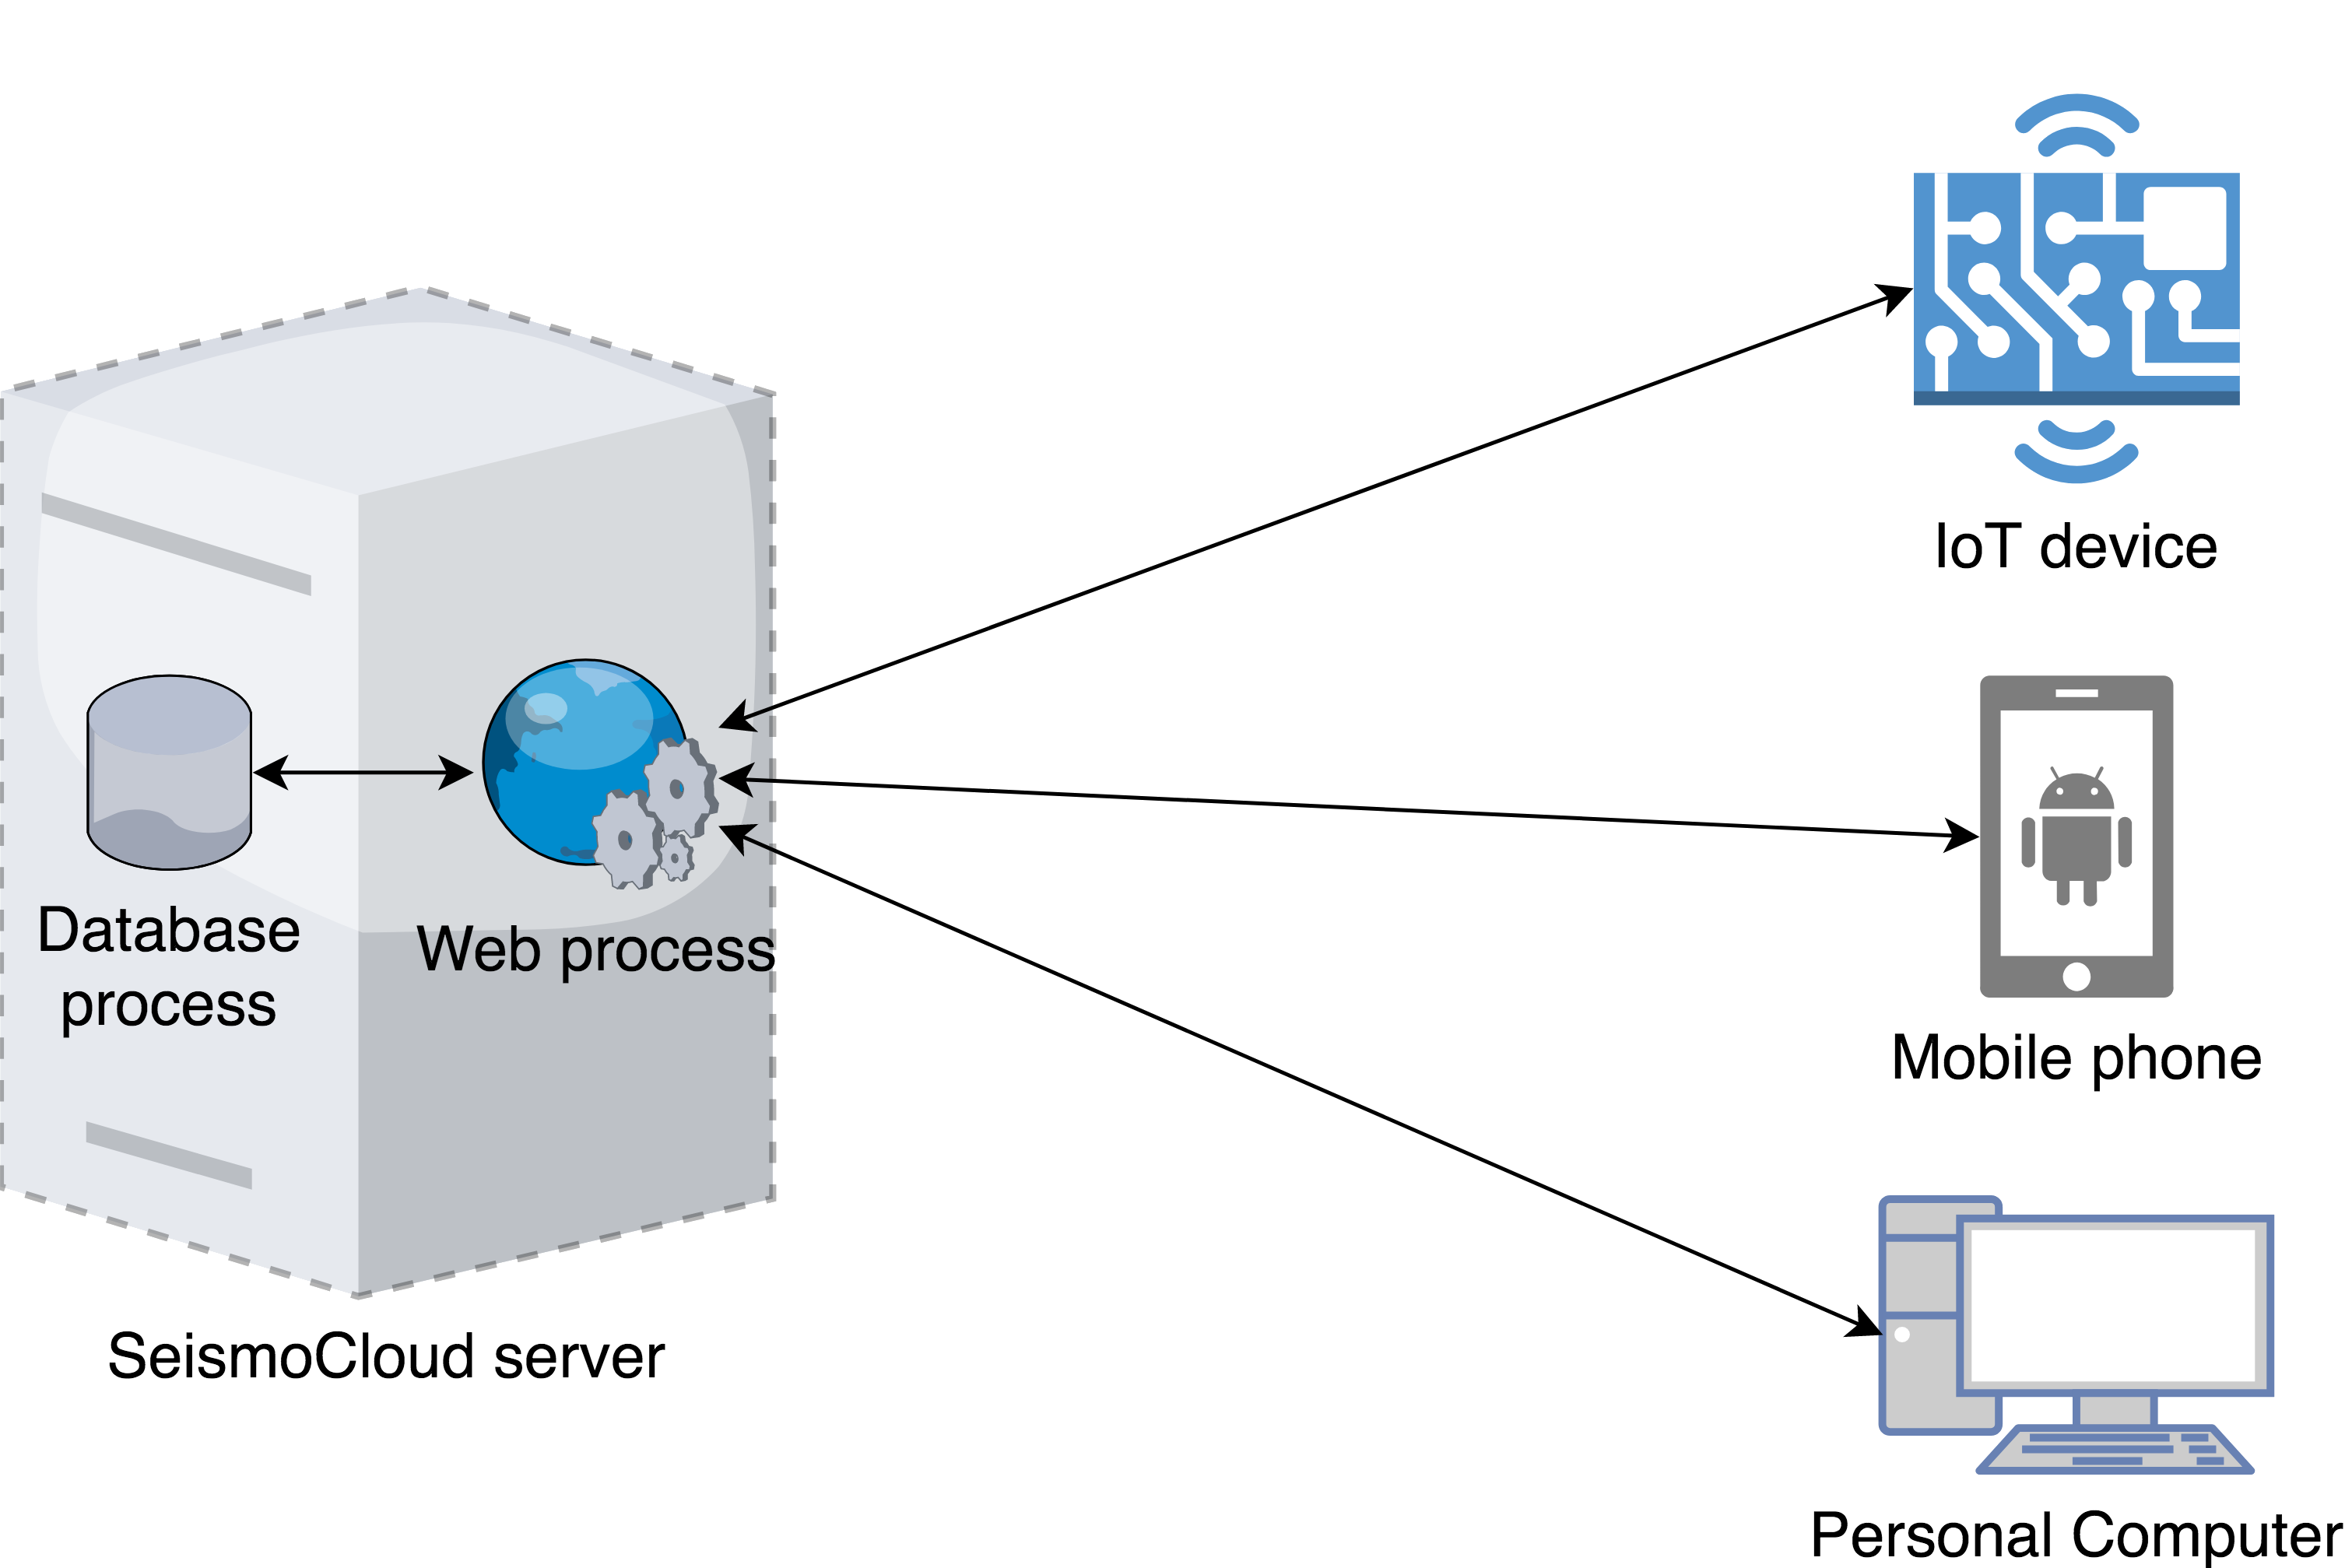
\includegraphics[width=0.8\textwidth]{scs-current-architecture}
\end{frame}


\begin{frame}{Current SeismoCloud architecture: numbers}
\begin{itemize}
  \item \textbf{Users}: \circa 13k devices, nearly 10k users
  \item \textbf{Wide area}: wide adoption in the EU, Mexico, west coast of US
  and south America
  \item \textbf{Computing power}: 2 x 2.4 GHz Intel CPU, avg load \circa 60\%
  \item \textbf{Memory}: 5 GB of RAM, avg load \circa 80\%
  \item \textbf{Storage}: +20 GB (both current and historical data)
  \item \textbf{Cost}: \circa 1400 € per year (server maintenance is made by us)
\end{itemize}

\textbf{Data collected in a quiet situation - eg. no major earthquakes}
\end{frame}


\begin{frame}{Current SeismoCloud architecture: map}
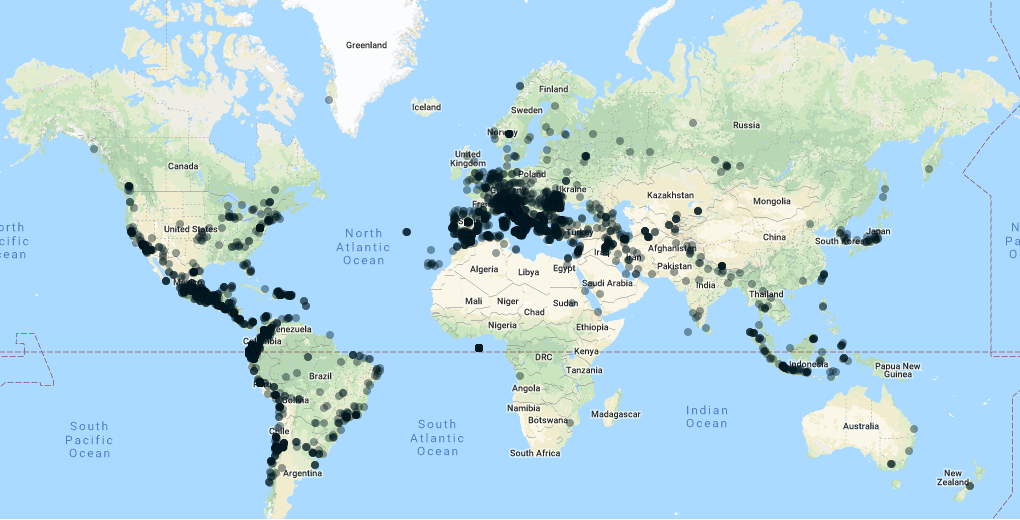
\includegraphics[width=\textwidth]{seismocloud_network}
\end{frame}


\begin{frame}{Current SeismoCloud architecture: issues}
\begin{itemize}
  \item \textbf{Limited scalability}: only vertical scalability. There is no way
  to scale the system horizontally due design flaws
  \item \textbf{No elasticity}: the system cannot adapt automatically to match
  workload changes over time
  \item \textbf{No high availability}: only one server manages (nearly) all. If
  it's down, the project is gone
  \item \textbf{Under provisioning}: the system is highly under-provisioned:
  necessary resources to handle a big network activity (such as a big earthquake)
  are missing
  \item \textbf{Over provisioning}: the system is over-provisioned for quiet
  periods of time (eg. no earthquakes)
\end{itemize}
\end{frame}


\begin{frame}{Current SeismoCloud architecture: improvements}
	A recent study highlighted the fact that HTTP(s) is not the right protocol to
	run a system like SeismoCloud, due many technical facts. The same study suggests
	to implement a \textit{Message-based, Publish-Subscription} protocol like
	\textbf{MQTT}, Message Queue Transport Protocol.

	\vspace{1em}

	The MQTT protocol needs a specialized software, named \textit{MQTT Broker}.
	The \textit{MQTT Broker} software needs to run in a server, and it will become
	vital for the project.

	\vspace{1em}

	Also, a gateway between MQTT and HTTP needs to be written from scratch: we named
	it \textit{SeismoCloud controller}. Even the \textit{SeismoCloud controller}
	will be part of the vital components.

\end{frame}



\section{Transforming SeismoCloud to be cloud-ready}

\begin{frame}{First step: Split components and dockerize}
We have three different components with different requirements:

\begin{itemize}
  \item \textbf{SeismoCloud core} (MQTT broker, SeismoCloud controller, database):
  high availability, high elasticity and geo-distributed, \textit{high priority}
  \item \textbf{API}: high availability and scalability
  \item \textbf{Website}: scalability, \textit{low priority}
\end{itemize}

They have been separated and re-written as stateless Docker containers. This is
a strategic decision in order to simplify the cloud deployment and multi-tier.
\end{frame}


\begin{frame}{First step: Split components and dockerize}
\centering
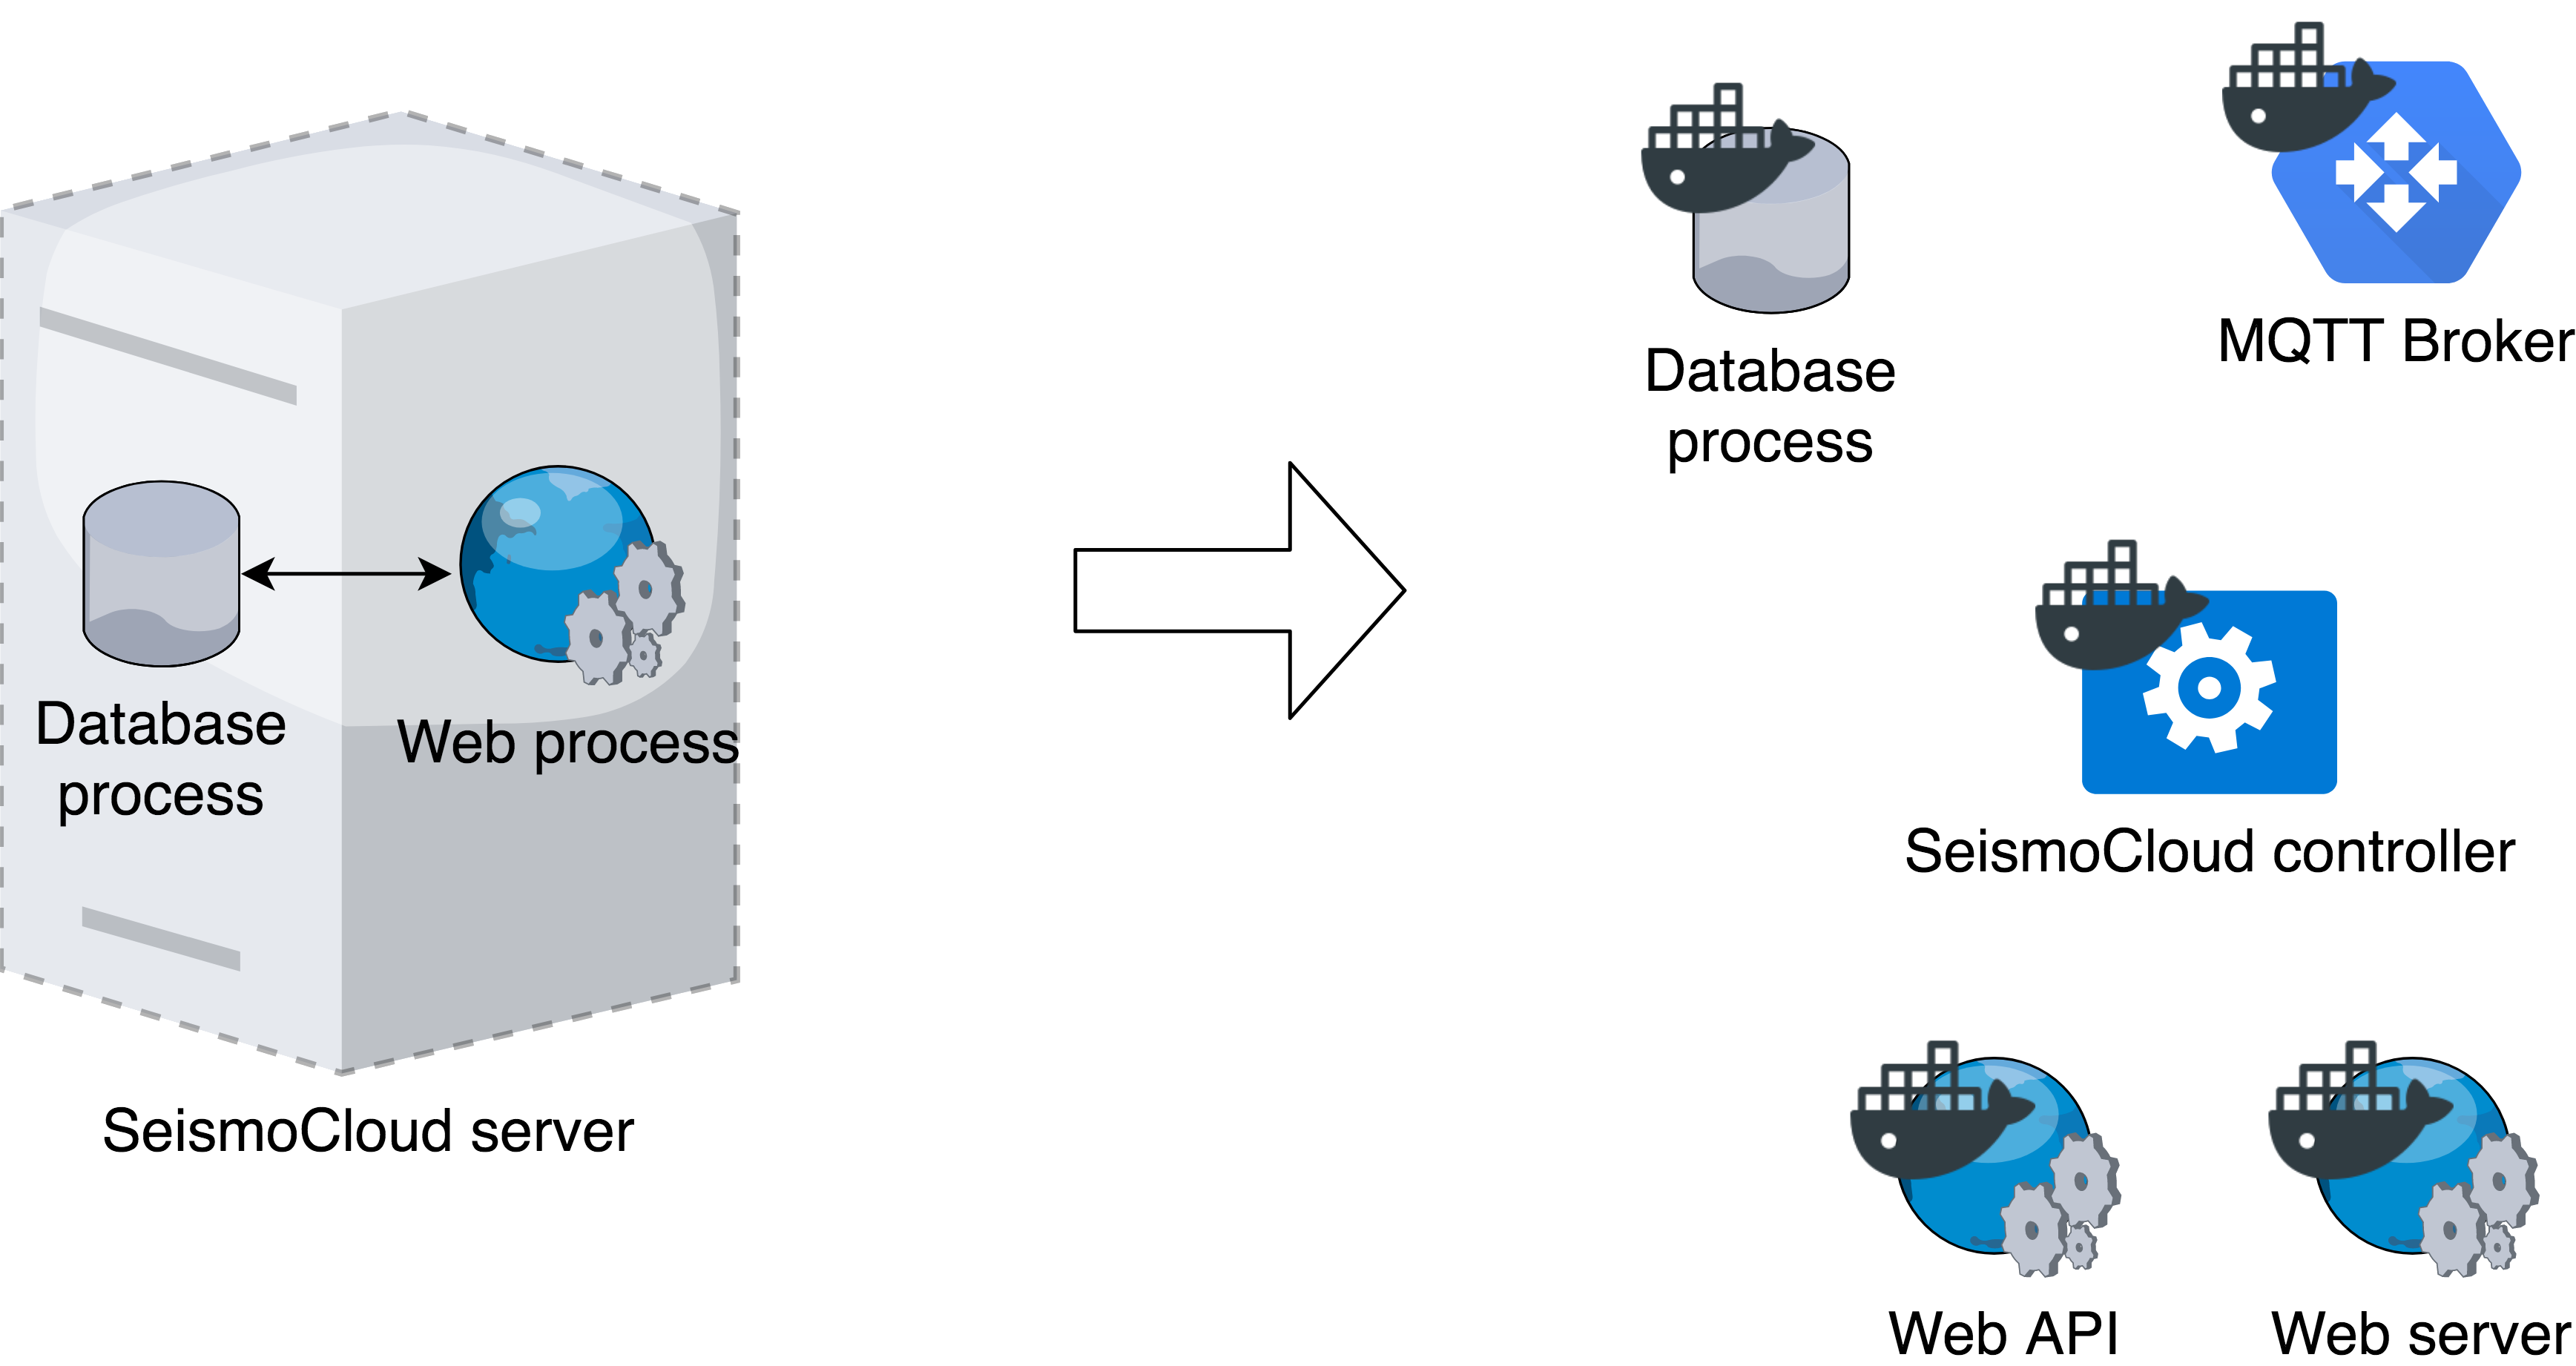
\includegraphics[width=0.9\textwidth]{scs-split-components}
\end{frame}


\begin{frame}{Second step: From MySQL to...}
A \textbf{core} component of SeismoCloud system is the data storage. We store
both technical data (eg. IoT device informations) and sensor data (such as
strongness of seismic wave acceleration).

The current system is based on a Relational DMBS named \textit{MySQL}.

As every R-DBMS, its capability to scale is very limited due to CAP theorem: a
R-DBMS prioritize \textit{Consistency} over \textit{Availability} during a
\textit{Partition}.
\end{frame}


\begin{frame}{CAP theorem}
\centering
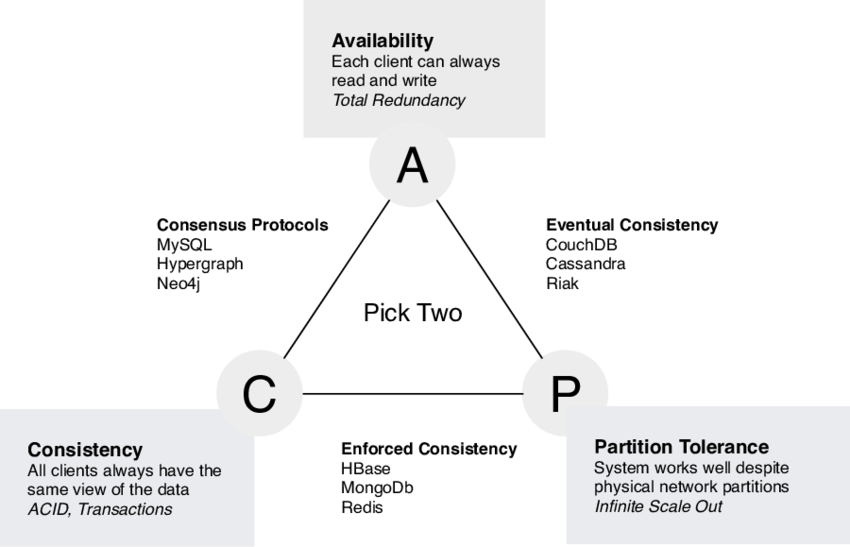
\includegraphics[keepaspectratio=true,width=\textwidth]{CAP-Theorem}
\end{frame}


\begin{frame}{Second step: From MySQL to Apache Cassandra / Redis}
For some storage \textit{actions} we need a highly scalable system that
doesn't need to be consistent at every moment. Examples of these situation are:

\begin{itemize}
  \item Store \textit{historical} data about earthquake waves
  \item Store device performance data
  \item Handle system and device logging
  \item Handle volatile data (such as session databases)
\end{itemize}

This needs are addressed with NoSQL products named \textit{Apache Cassandra} and
\textit{Redis}.
\end{frame}


\begin{frame}{Future SeismoCloud architecture}
\centering
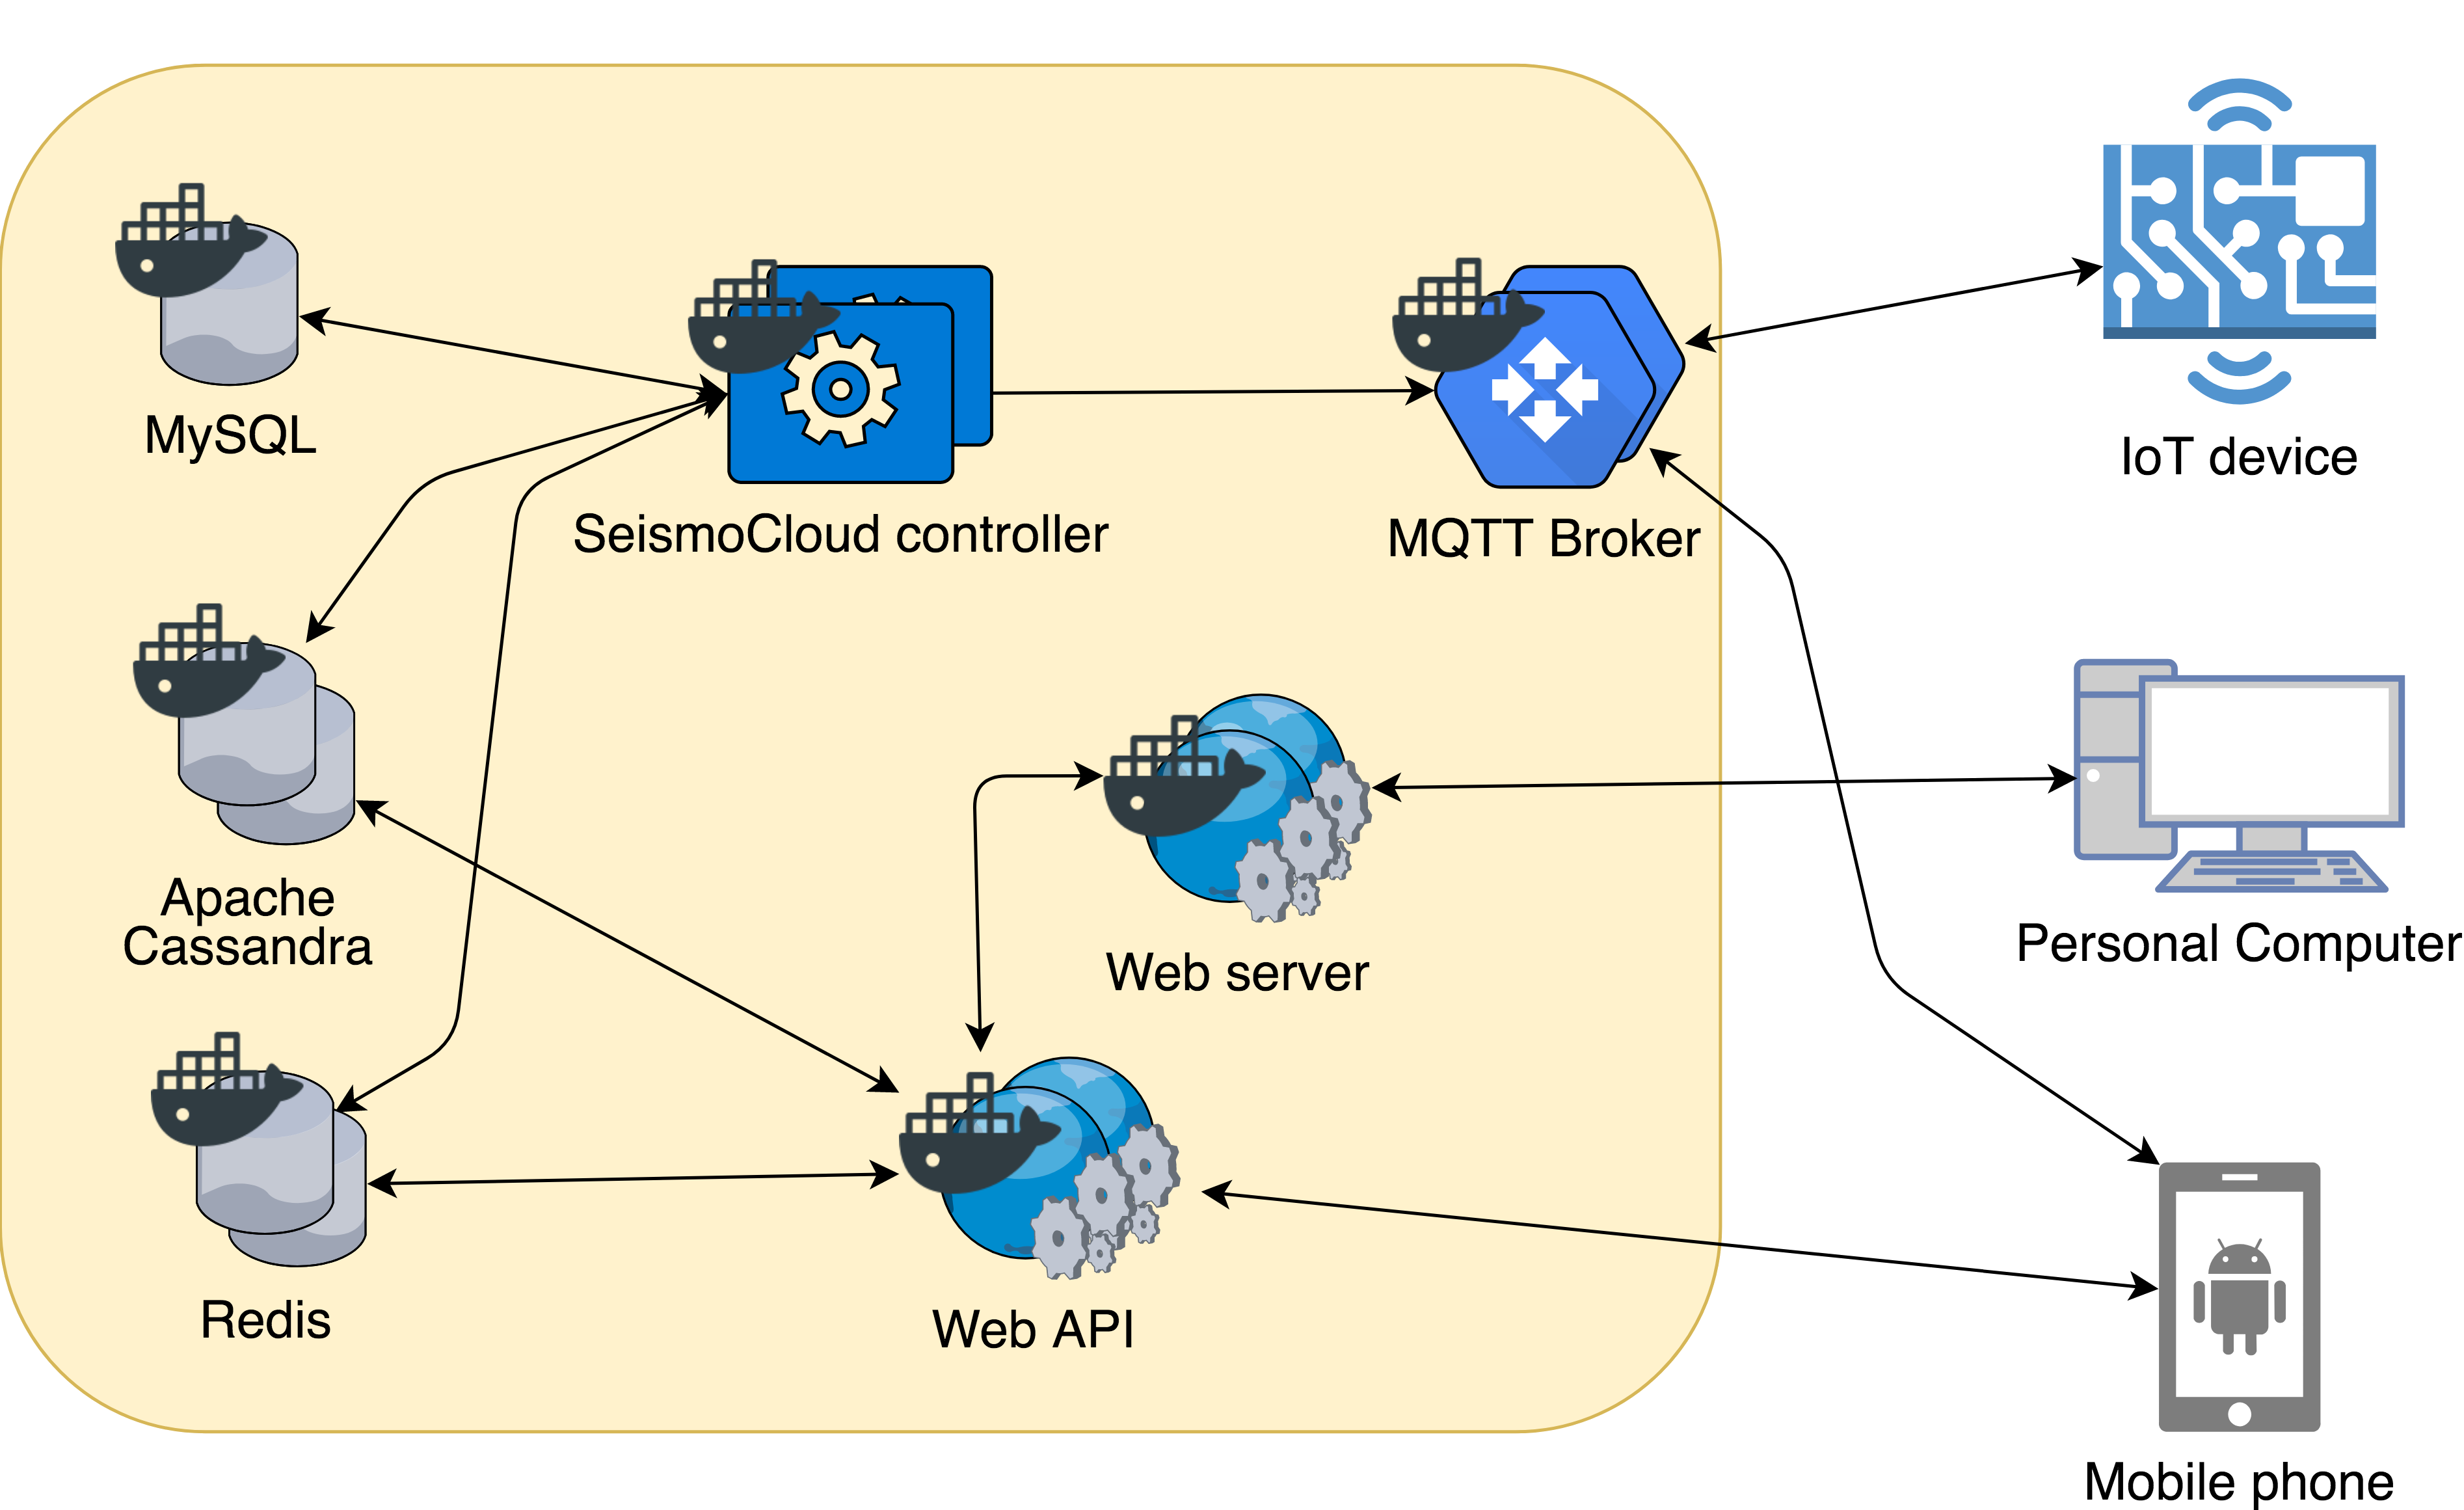
\includegraphics[keepaspectratio=true,width=\textwidth]{scs-future-architecture}
\end{frame}


\begin{frame}{Refactoring costs}

	The overall refactoring took nearly a month of a 1-person development, and will
	require an estimated time of 2 week of testing (before going into production).

	\vspace{3em}

	The total estimated cost for this operation is 7500 € (250 € / workday)

\end{frame}



\section{Moving to the Cloud}

\begin{frame}{OpenShift}
\textbf{OpenShift} is an open-source container system from
\textbf{Red Hat}. It supports \textit{Docker} containers natively using
\textit{Kubernetes} (a container \textit{orchestrator} from Google).

OpenShift can be used both \textit{on-premise} (even for free) or
\textit{online} (using Red Hat's own cloud).

OpenShift enables \textit{Platform-as-a-Service} cloud.

\centering
\vspace{1em}

\includegraphics[keepaspectratio=true,height=40pt]{openshift_logo}
\hspace{1em}

\includegraphics[keepaspectratio=true,height=40pt]{docker_logo}
\end{frame}


\begin{frame}{OpenShift}
\centering
\hspace*{-0.4in}
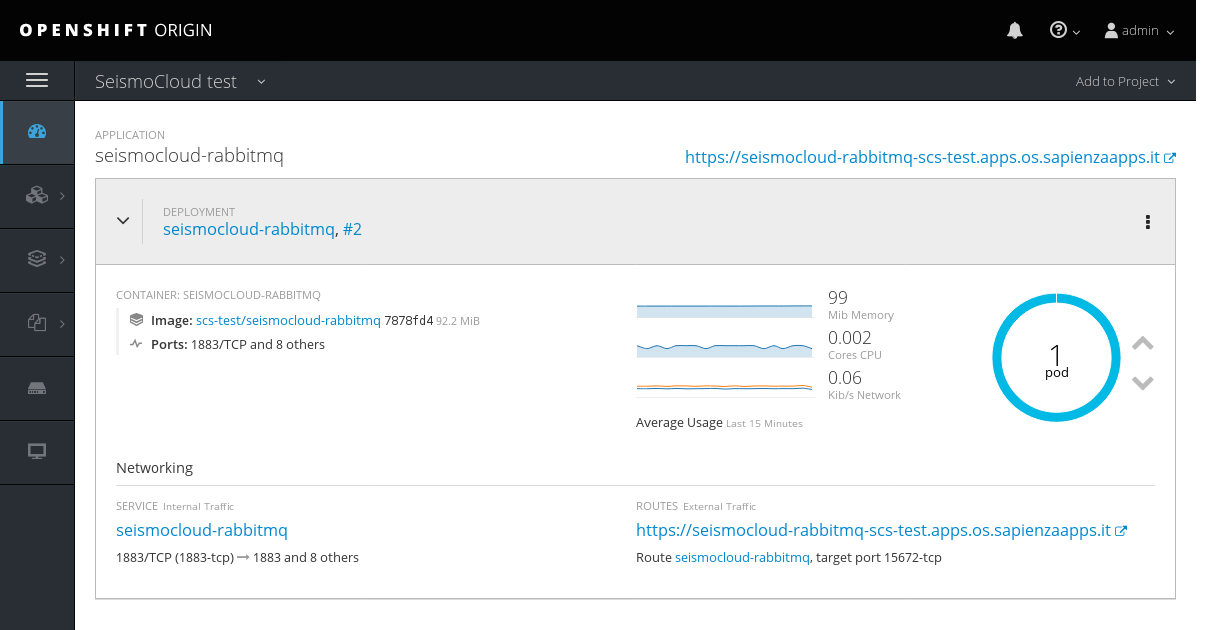
\includegraphics[width=1.19\textwidth]{openshift}
\end{frame}


\begin{frame}{PaaS advantages}
By deploying this project on Red Hat's OpenShift cloud, we have:

\begin{itemize}
  \item \textbf{High availability}: Red Hat has many datacenter, and OpenShift
  is capable to power up pods in different sites around the globe. Also it uses
	Amazon AWS to load-balacing its own servers (\textit{Hybrid IaaS}).
  \item \textbf{High elasticity}: the underlying Kubernetes is able to scale
  automatically based on resource usages (eg. CPU/memory) and/or external
	triggers (such as the application itself)
	\item \textbf{Pay-per-use}: we'll pay per-use, so costs will grow as the user
	base grow, and we'll be able to react to usage peaks (earthquakes)
\end{itemize}
\end{frame}




\begin{frame}{PaaS multi-tiering}

By using Docker we'll be able to have a \textbf{multi-tier} architecture:
many cloud providers supports Docker containers (such as Amazon EC2, Google
Cloud, IBM Bluemix) as a backup, load balacing or as new main cloud provider in
the future, with no changes to the code.

\begin{center}

\includegraphics[width=0.5\textwidth]{amazon_ec2}
\end{center}


In fact, in this (\textit{testing}) phase, we have an hybrid cloud system:
we have both \textit{on-premise} and \textit{on-cloud} OpenShift instances, and
some plain Docker containers in the production server \textbf{deployed with the
same Docker images}.

\end{frame}



\begin{frame}{Old vs PaaS: costs and SLA}

Recap of conditions for the current architecture:

\begin{itemize}
  \item \textbf{Costs (yearly)}: \circa 1400 €
  \item \textbf{SLA} (server+net): 99.00\% (\circa 7.5 hours per month)
  \item \textbf{Maintenance}: software/O.S. maintenance is our duty
  \item \textbf{No HA, no scalability, no redundancy}
\end{itemize}

With OpenShift \textit{Platform-as-a-Service} and new architecture:

\begin{itemize}
  \item \textbf{Costs (yearly)}: \circa 1000 € at \textbf{idle}, plus
	\textbf{one-time cost} of 7500 €
  \item \textbf{SLA} (PaaS+net): from 99.00\% to 99.99\% (\circa 4 minutes)
  \item \textbf{Maintenance}: software/O.S. maintenance is offloaded
  to the PaaS provider - we need to maintain only our own software
  \item \textbf{HA, scalability, elasticity, ...}
\end{itemize}

\end{frame}



\begin{frame}[standout]
  \Huge Questions?
\end{frame}

\begin{frame}{}
  \begin{center}\ccbysa\end{center}

  \small This presentation is available on GitHub as LaTeX source and compiled PDF: \\
  \url{https://github.com/Enrico204/cloud-symposium-seismocloud}
\end{frame}

\end{document}
